\subsection{Index Overview}
\label{indexIntro}
The CL-tree index is built based on the key observation that cores are nested.
Specifically, a $(k$+1$)$-$\widehat {core}$ must be contained in a $k$-$\widehat{core}$.
The rationale behind is, a subgraph has a minimum degree at least $k+1$ implies that
it has a minimum degree at least $k$. Thus, all $k$-$\widehat {core}$s can be organized into a tree structure\footnote{We use ``node'' to mean ``CL-tree node'' in this paper.}. We illustrate this in Example~\ref{eg:index}.

\begin{example}
\label{eg:index}
Consider the graph in Figure~\ref{fig:kcoreGraph}.
All the $k$-$\widehat {core}$s can be organized into a tree as shown in Figure~\ref{fig:ucktree}.
The height of the tree is 4.
For each tree node, we attach the core number and vertex set of its corresponding $k$-$\widehat {core}$.
\end{example}

From the tree structure in Figure~\ref{fig:ucktree}, we conclude that,
if a ($k$+1)-$\widehat {core}$ (denoted as ${\mathcal C}_{k+1}$)
is contained in a $k$-$\widehat {core}$ (denoted as ${\mathcal C}_k$),
then there is a tree node corresponding to ${\mathcal C}_{k+1}$ and its parent node corresponds to ${\mathcal C}_k$.
Besides, the height of the tree is at most $k_{max}+1$, where $k_{max}$ is the maximum core number.

\begin{figure}[ht]
    \centering
    \mbox{
        \subfigure[tree structure]{
            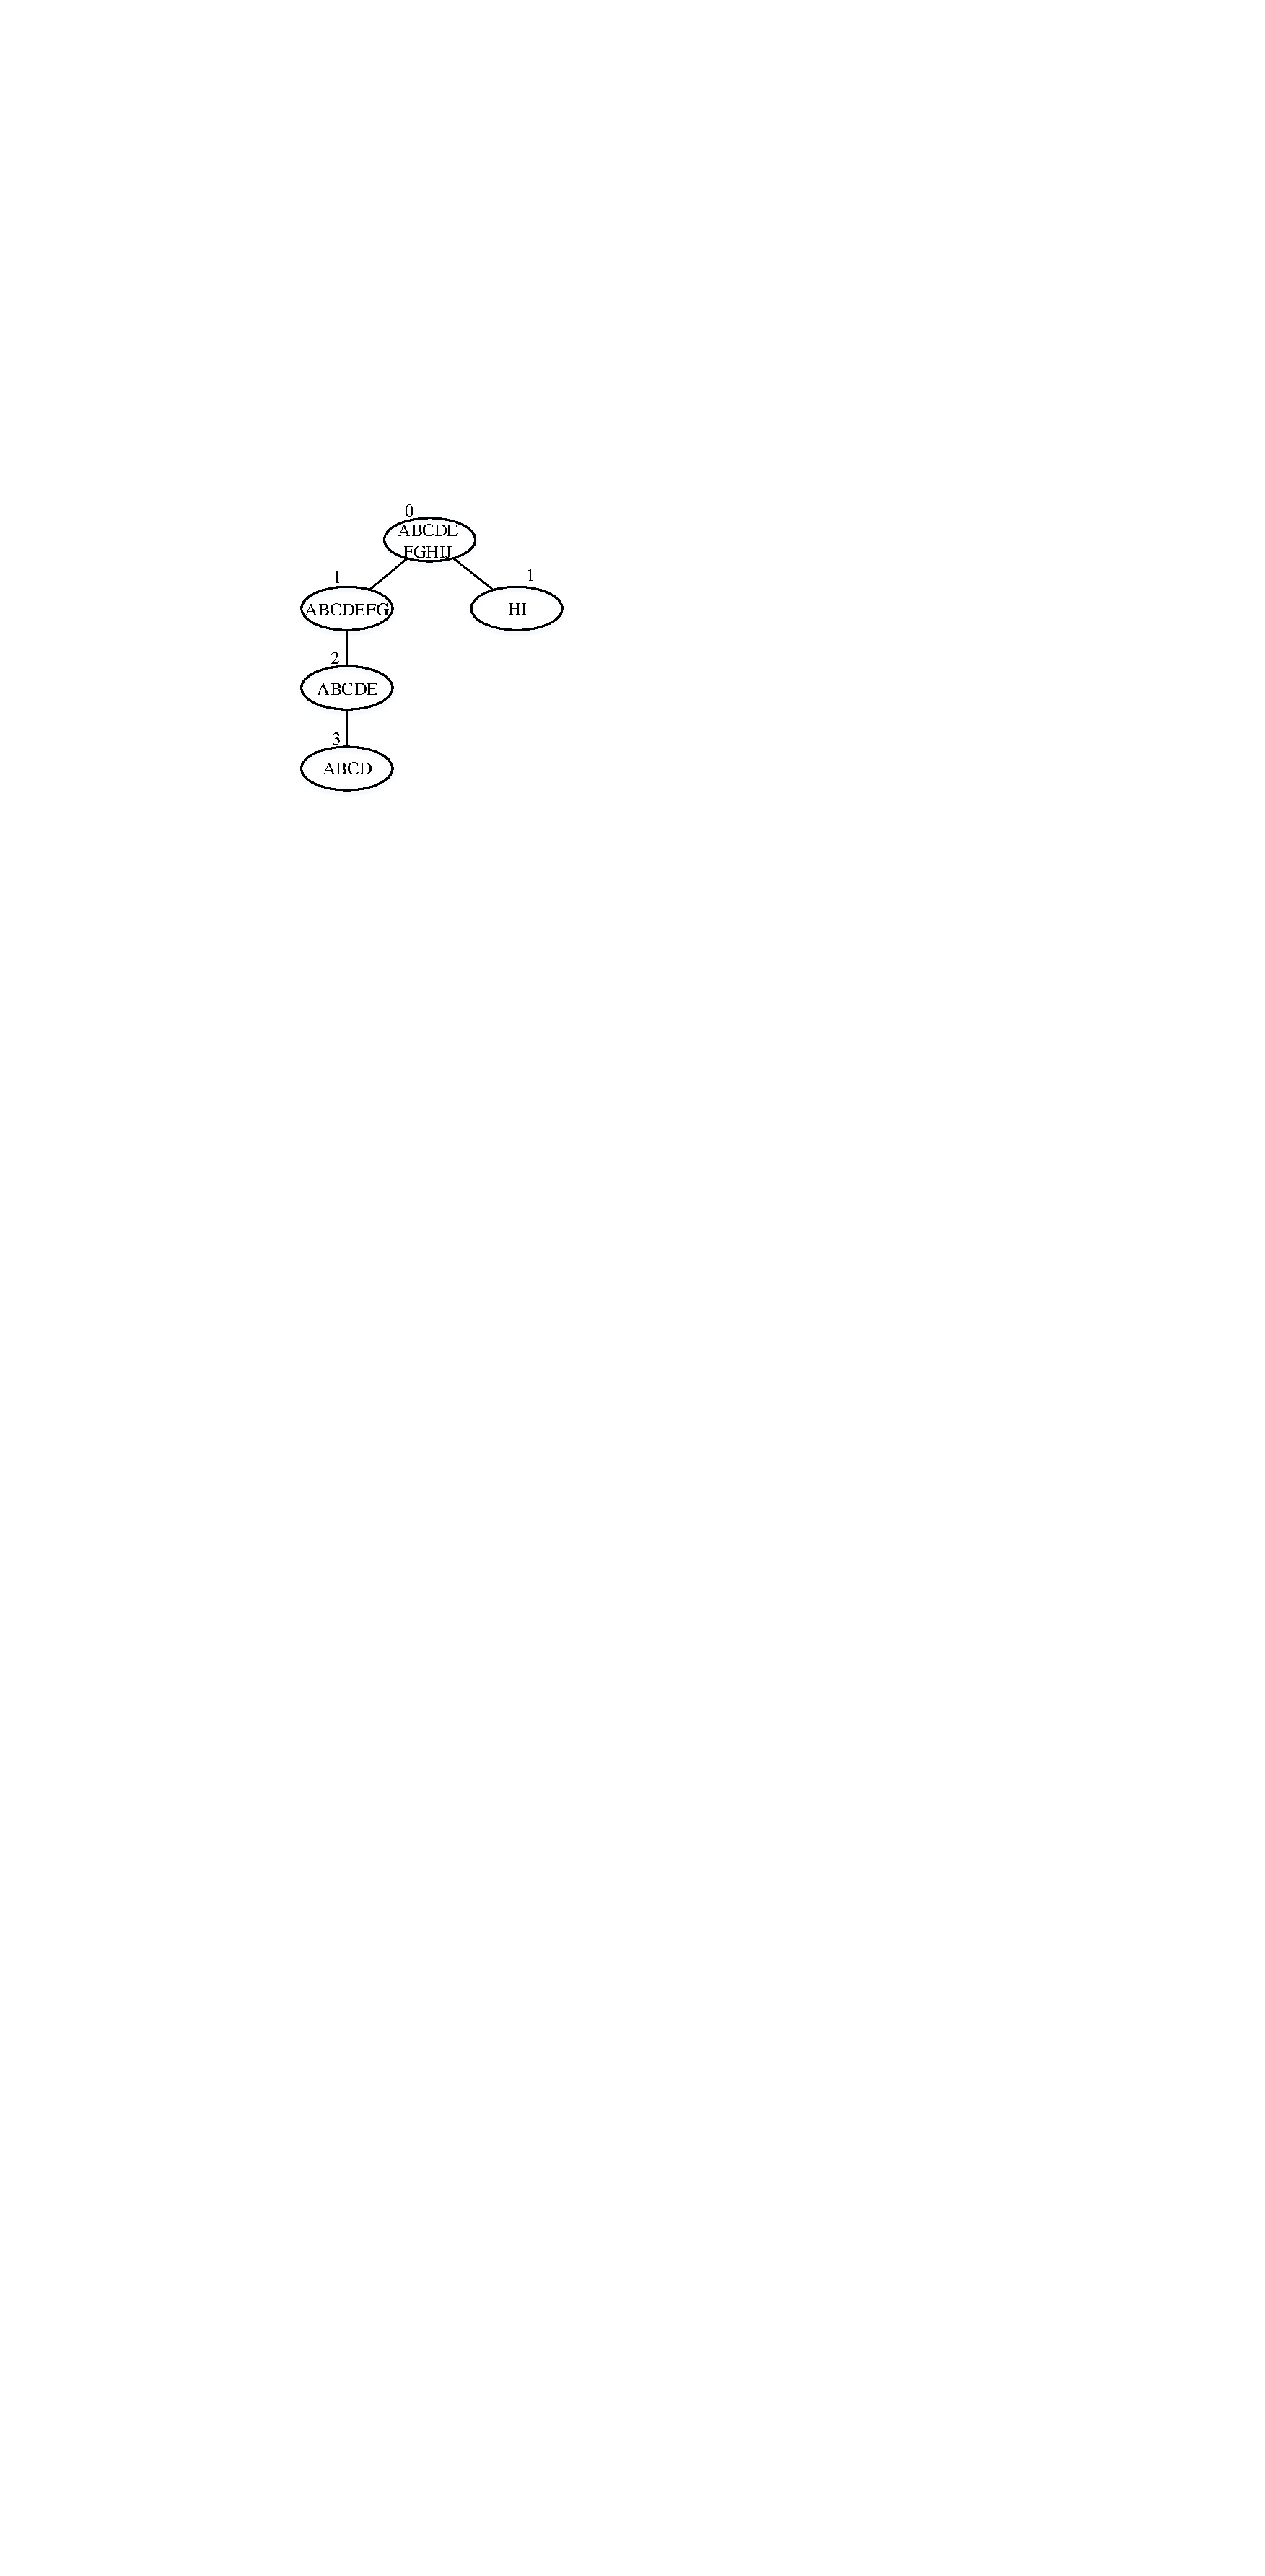
\includegraphics[width=.375\columnwidth]{figures/uck-tree}
            \label{fig:ucktree}
        }
        \hspace{2ex}
        \subfigure[CL-tree index]{
            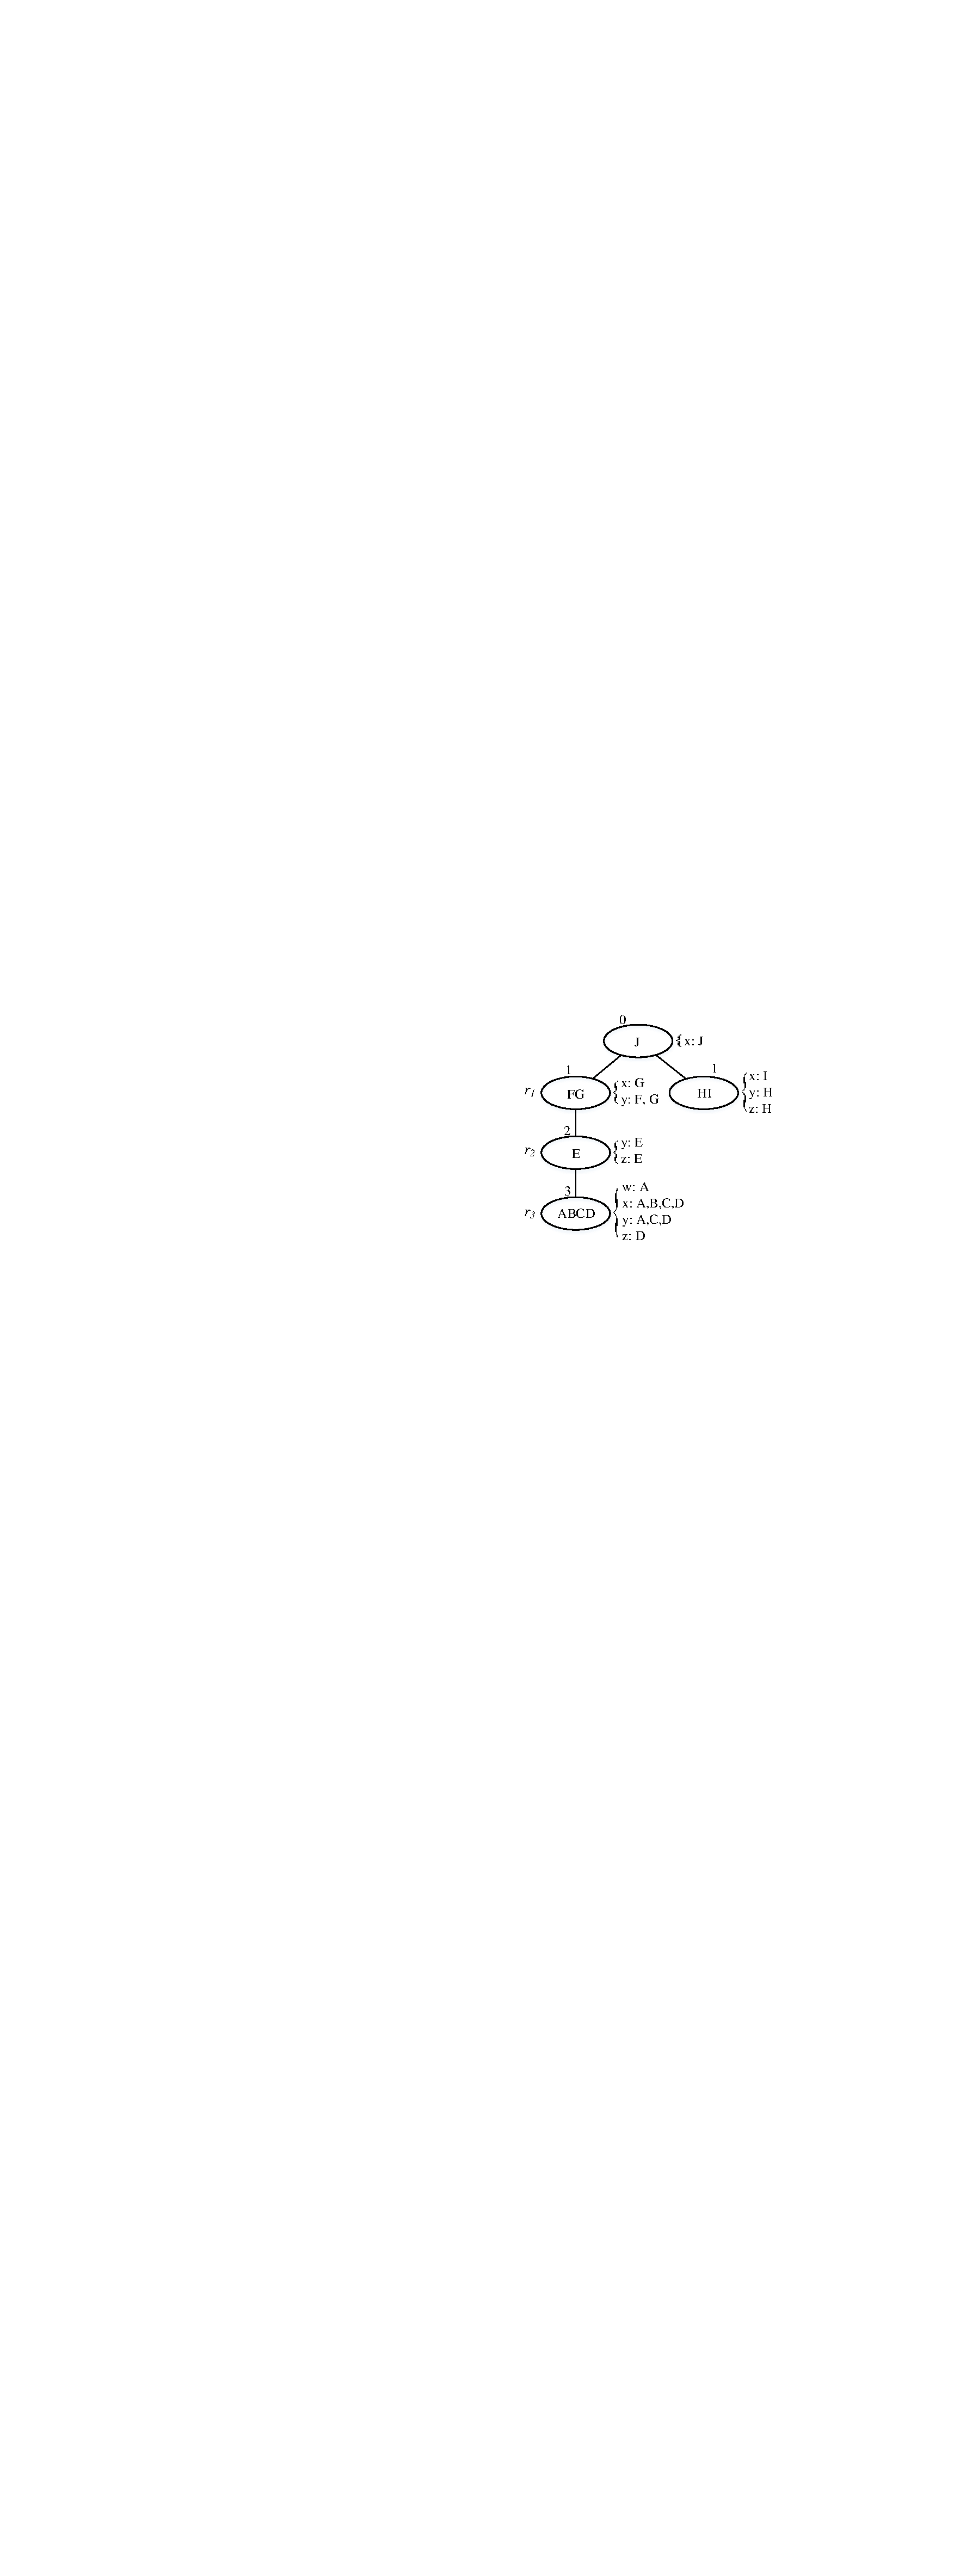
\includegraphics[width=.45\columnwidth]{figures/ck-tree}
            \label{fig:cktree}
        }
    }
    \caption{An example CL-tree index.}\label{fig:index}
\end{figure}

The tree structure in Figure~\ref{fig:ucktree} can be stored compactly, as shown in Figure~\ref{fig:cktree}.
The key observation is that, for any internal node $p$ in the tree,
the vertex sets of its child nodes are the subsets of $p$'s vertex set,
because of the inclusion relationship. To save space cost,
we can remove the redundant vertices that are shared by $p$'s child nodes from $p$'s vertex set.
After such removal, we obtain a compressed tree,
where each graph vertex appears only once.
This structure constitutes the CL-tree index, the nodes of which are further augmented by inverted lists (Figure~\ref{fig:cktree}).
For each keyword $e$ that appears in a CL-tree node, a list of IDs of vertices whose keyword sets contain $e$ is stored.  For example, in node $r_3$, the inverted list of keyword $y$ contains $\{A,C,D\}$. As discussed later, given a keyword set $T$, these inverted lists allow efficient retrieval of vertices whose keyword sets contain $T$.
To summarize, each CL-tree node contains five elements:

$\bullet$ \emph{coreNum}: the core number of the $k$-$\widehat {core}$;

$\bullet$ \emph{vertexSet}: a set of graph vertices;

$\bullet$ \emph{invertedList}: a list of $\textless key,value\textgreater$ pairs, where the $key$ is a keyword contained by vertices in $vertexSet$ and the $value$ is the list of vertices in $vertexSet$ containing $key$;

$\bullet$ \emph{childList}: a list of child nodes.

\chen{
$\bullet$ \emph{fatherNode}: the father node of the current node.
}

Figure~\ref{fig:cktree} depicts the CL-tree index for the example graph in Figure~\ref{fig:kcoreGraph},
the elements of each tree node are labeled explicitly.
Using the CL-tree, the following two key operations used by our query algorithms (Section~\ref{query}), can be performed efficiently.

$\bullet$ {\bf{Core-locating.}} Given a vertex $q$ and a core number $c$,
	find the $k$-$\widehat {core}$ with core number $c$ containing $q$,
	by traversing the CL-tree.
	
$\bullet$ {\bf{Keyword-checking.}} Given a $k$-$\widehat {core}$, find vertices which contain a given keyword set, by intersecting the inverted lists of keywords contained in the keyword set.


\textbf{Remarks.}
The CL-tree can also support $k$-$\widehat {core}$ queries on general graphs without keywords.
For example, it can be applied to finding $k$-$\widehat{core}$ in previous community search methods~\cite{KDD2010}.


\textbf{Space cost.}
Since each graph vertex appears only once and each keyword only needs constant space cost,
the space cost of keeping such an index is $O({\widehat l}\cdot n)$,
where $\widehat l$ denotes the average size of $W(v)$ over $V$.
Thus, the space cost is linear to the size of $G$. 